\documentclass[a4paper,11pt]{article}
\usepackage[T1]{fontenc}
\usepackage[utf8]{inputenc}
\usepackage{lmodern}
\usepackage{hyperref}
\usepackage{graphicx}
\usepackage[english]{babel}

\title{\Huge \textbf{Metody analýzy dat}  
\\ \huge Analýza videoherního průmyslu }
\author{\textsc{Ondřej Řeháček (REH0063)}}
\begin{document}
\maketitle

\section{Dataset}
Dataset obsahuje statistické informace o prodeji více než 16 tisíců nejprodávanějších videoherních titulů v rozdilných regionech. Je volně dostupný na keggle.com a byl publikován Gregory Smithem 10.Října 2016. Obsahuje tedy poměrně aktuální data čerpána z ověřeného zdroje ve videoherním světě - vgchartz.com, pomocí Python skriptu \footnote{https://github.com/GregorUT/vgchartzScrape}. pro sběr dat z této webové stránky 

\subsection{Motivace}
Videoherní průmysl je již stejně dominantní jako filmový či hudební. Postupem času s vývojem techniky se vyvíjí i tato forma zábavy a v dnešní době mohou videohry vyprávět stejně komplexní příběhy jako celovečerní filmy. Není žádným tajemstvím, že jednotlivé kontinenty májí podstatně jinak rozložený prodej a zájem o videohry. S pomocí tohoto datasetu a jeho analýzy chci tyto rozdíly zdokumentovat a detailně popsat.

\subsection{Atributy}
\begin{tabular}{|c|l|}
\hline
\textbf{Rank} & Pořadí titulu v počtu prodejů. \\ \hline
\textbf{Name} & Název herního titulu \\ \hline
\textbf{Platform} & Platforma na které titul běží. \\ \hline
\textbf{Year} & Rok vydání hry. \\ \hline
\textbf{Genre} & Žánr herního titulu. \\ \hline
\textbf{Publisher} & Vydavatel / Vývojář titulu. \\ \hline
\textbf{NA\_Sales} & Prodeje na území státu serevní ameriky. (V miliónech) \\ \hline
\textbf{JP\_Sales} & Prodeje na území Japonska. (V miliónech) \\ \hline
\textbf{EU\_Sales} & Prodej na území státu Evropy. (V miliónech) \\ \hline
\textbf{Other\_Sales} & Prodej na území zbylých státu. (V miliónech) \\ \hline
\textbf{Global\_Sales} & Celkový počet prodaných kusů. \\ \hline
\end{tabular}


\subsection{Úpravy a chybějící data}
Přibližně 27 titulů bylo opraveno, protože obsahovaly nesmyslné hodnoty. Původně je v datasetu asi 329 položek, které nemají kompletní data - jedná se převážně o chybějící rok vydání. Některé z položek byly manuálně doplněny o zjišťěná data.

\subsection{Otázky, pro které hledáme odpověďi.}

Kromě obecné analýzy dat, hledáme odpovědi na následující specifičtější otázky:

\begin{itemize}
\item Jak se zvětšoval videoherní trh s postupem času ?

\item Jaké jsou oblíbené žánry titulů v rozdilných regionech ?

\item Jaké platformy byly nejuspěšnějí ve svých generacích ?

\item Které žánry byly nejdominantnější na určitých platformách ?

\item Které žánry jsou nejdominantnější v určitých regionech ?

\item Preferují určité regiony rozdilné vývojáře ?
\end{itemize}

\subsection{Analýza}
Analýza datasetu je provedena v R (IDE RStudio 1.0.44) a byly využity následující baliky:

\begin{itemize}
\item dplyr

\item ggplot2

\item dplyr

\item scales

\item reshape2
\end{itemize}

\newpage

\section{Obecná analýza}


\subsection{Analýza atributů}
\begin{center}
\begin{tabular}{|c|c|c|c|c|c|}
\hline
\textbf{}              & \textbf{Length} & \textbf{Min} & \textbf{Mean} & \textbf{Max} & \textbf{Type} \\ \hline
\textbf{Rank}          & 16600           & 1            & 8300          & 16600        & Integer       \\ \hline
\textbf{Name}          & X               & X            & X             & X            & String        \\ \hline
\textbf{Platform}      & X               & X            & X             & X            & String        \\ \hline
\textbf{Year}          & 16600           & 1980         & 1993          & 2016         & Mixed         \\ \hline
\textbf{Genre}         & X               & X            & X             & X            & String        \\ \hline
\textbf{Publisher}     & X               & X            & X             & X            & String        \\ \hline
\textbf{NA\_Sales}     & 16600           & 0.0000       & 0.2647        & 41.4900      & Float         \\ \hline
\textbf{EU\_Sales}     & 16600           & 0.0000       & 0.1467        & 29.0200      & Float         \\ \hline
\textbf{JP\_Sales}     & 16600           & 0.0000       & 0.0778        & 10.2200      & Float         \\ \hline
\textbf{Other\_Sales}  & 16600           & 0.0000       & 0.0480        & 10.5700      & Float         \\ \hline
\textbf{Global\_Sales} & 16600           & 0.0000       & 0.5374        & 82.7400      & Float         \\ \hline
\end{tabular}
\end{center}


\subsection{Počet titulů na rok.}

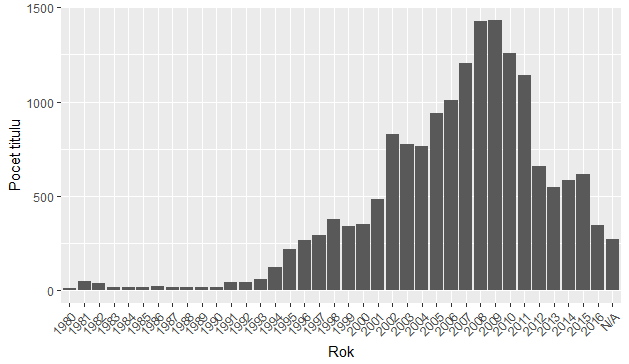
\includegraphics[scale=0.8]{Rplot}

\begin{itemize}
\item Nárust v roce 1994 po dostupnosti \textbf{Sony Playstation (102 mil.)}

\item Po roce 2001, kdy se na trh dostává historicky nejprodávanější konzole Sony \textbf{Playstation 2 (> 155 mil.)}.

\item V letech 2005-2011 najdeme hodnoty nejvyšší, vzhledem k tomu, že trh ovládá \textbf{Nintendo DS (154 mil.)} , \textbf{Nintendo Wii (101 mil.)}, \textbf{Xbox 360 (85 mil.)}, \textbf{Playstation 3 (84 mil.)}  najednou - všechny astronomicky úspěšné produkty.
\end{itemize}


\newpage

\subsection{Rozložení platforem}

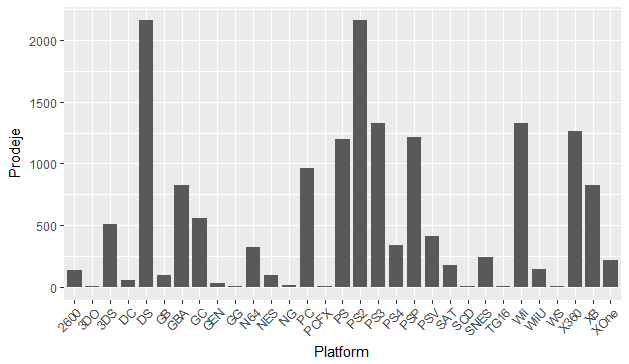
\includegraphics[scale=0.75]{Rplot03}

Zde lze potvrdit tvrzení uvedené u grafu 2.1. Jasně dominují právě ty nejlépe prodávané platformy, které mohou za nárůsty umístěných titulů v době kdy byly uvedeny a prodávány. 



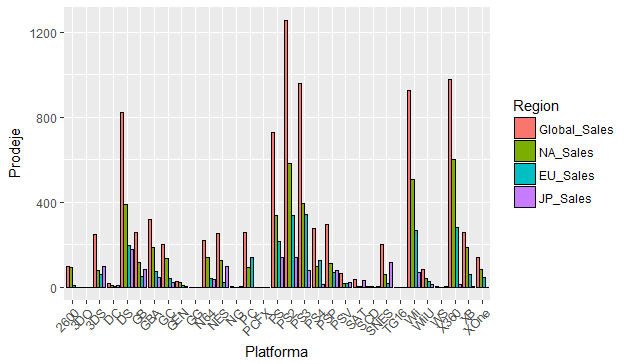
\includegraphics[scale=0.9]{Rplot02}

Také se projevuje preference jednotlivých regionu - Sony ze svou řadou Playstation jasně ovládá domovský japonský trh společně s Nintendem, naopak značka Xbox od Microsoftu je v Japonsku naprostým propadákem. Na druhé straně v USA - domácí Xbox převládá nád ostatními konzolemi. Evropa je regionem "neutrálním".

\newpage

\subsection{Oblíbené žánry}

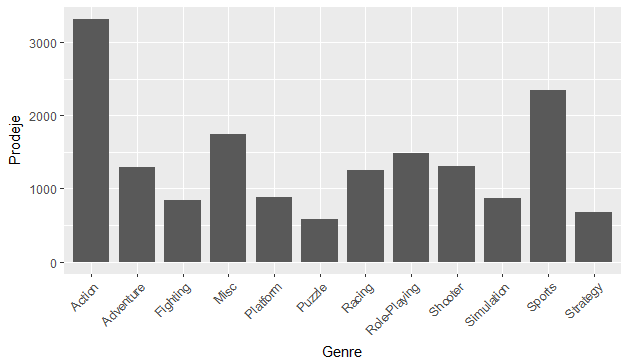
\includegraphics[scale=0.75]{Rplot04}

Nejoblíbenějším žánrem jsou akční hry. Na druhém místě doprovázeny sportovními hrami, které se uvádí na trh pravidelně každý rok a proto představují velkou část datasetu. Nejméně se vyskytují logické a strategické hry.


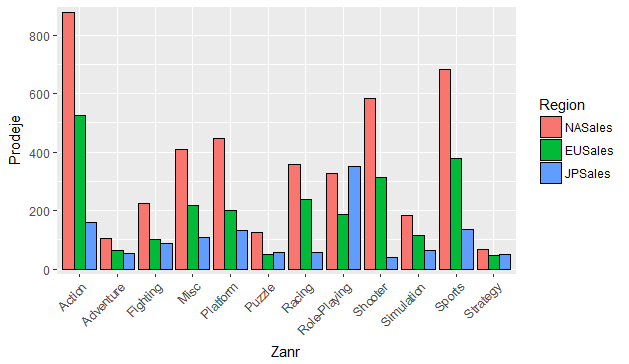
\includegraphics[scale=0.9]{Rplot06}

Při rozdělení prodejů jednotlivých žánru do regionu se opět projevují již "zajeté" předpoklady. Japonskému trhu vládnou RPG hry, jejiž převaha je na grafu velmi výrazná. Evropa a Severní amerika naopak preferuje hry akční a sportovní.

\newpage


\subsection{Vydavatelé a tituly podle regionu}

\subsubsection{Evropa}
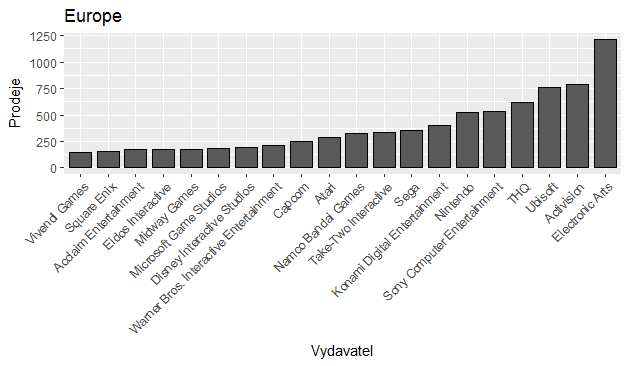
\includegraphics[scale=0.8]{Rplot10}

\begin{center}
\begin{tabular}{|c|c|}
\hline
\textbf{Název titulu}                   & \textbf{Prodeje v regionu (mil.)} \\ \hline
\textbf{Wii Sports}                     & 29.02                             \\ \hline
\textbf{Grand Theft Auto V}             & 23.04                             \\ \hline
\textbf{Mario Kart Wii}                 & 12.88                             \\ \hline
\textbf{FIFA 15}                        & 12.40                             \\ \hline
\textbf{Call of Duty: Modern Warfare 3} & 11.29                             \\ \hline
\end{tabular}
\end{center}

Evropu ovládá Electronic Arts díky sportovním seriim jako je FIFA, NHL, které jsou na územi EU velmi oblíbené a patří opakovaně k nejprodávanějším titulům. První místo v prodeji videoher patří Nintendu s Wii Sports, vzhledem k tomu, že byl po dlouhou dobu dodávan s každou konzolí v základním balení. Historický úspěch zaznamenál taky Rockstar Games se svým Grand Theft Auto V.


\newpage

\subsubsection{Severní Amerika}
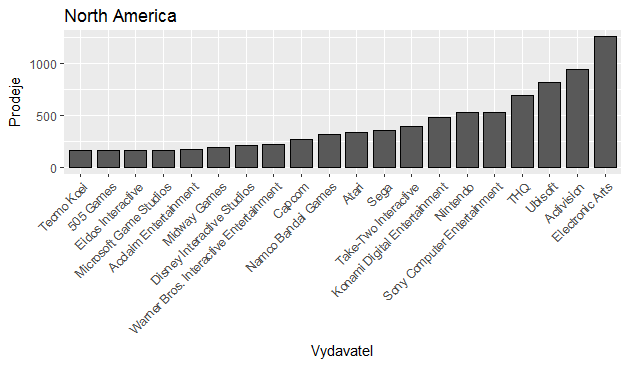
\includegraphics[scale=0.8]{Rplot11}

\begin{center}
\begin{tabular}{|c|c|}
\hline
\textbf{Název titulu}       & \textbf{Prodeje v regionu (mil.)} \\ \hline
\textbf{Nintendo Wii Sports}         & 41.49                             \\ \hline
\textbf{Super Mario Bros.}  & 32.48                             \\ \hline
\textbf{Duck Hunt}          & 26.93                             \\ \hline
\textbf{Tetris}             & 26.17                             \\ \hline
\textbf{Grand Theft Auto V} & 23.46                             \\ \hline
\end{tabular}
\end{center}

Stejně jako v EU, nejlépe se zde daří domácímu Electronic Arts a Activision díky herním značkám jako je akční Battlefield, Call of Duty či sportovní tituly série NFL. Historicky nejprodávanější tituly však patří společnosti Nintendo, vzhledem k expanzi do spojených států a dominanci jejich systému NES, SNES a Game Boy v průběhu 80 a 90 tých let na uzemí USA.

\newpage

\subsubsection{Japonsko}
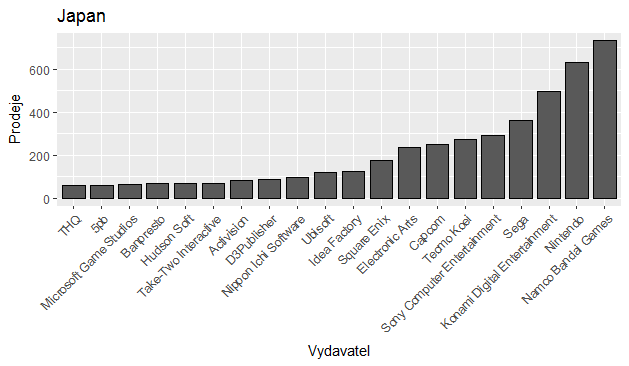
\includegraphics[scale=0.8]{Rplot12}

\begin{center}
\begin{tabular}{|c|c|}
\hline
\textbf{Název titulu}                  & \textbf{Prodeje v regionu (mil.)} \\ \hline
\textbf{Pokemon Red/Pokemon Blue}      & 10.22                             \\ \hline
\textbf{Pokemon Gold/Pokemon Silver}   & 7.20                              \\ \hline
\textbf{Super Mario Bros.}             & 6.96                              \\ \hline
\textbf{New Super Mario Bros.}         & 6.50                              \\ \hline
\textbf{Pokemon Diamond/Pokemon Pearl} & 6.04                              \\ \hline
\end{tabular}
\end{center}

Klasicky v Japonském regionu je situace úplně jiná. Je zde jasně vidět preferování lokálních značek jako je Namco, Nintendo, Konami, Square. Stejně tak je rozdilná sitace u nejprodavanějích titulech které kompletně patří domácímu Nintendu a značkám jako Pokémon a Super Mario Brothers.

\newpage


\section{Specifická analýza}

\subsection{Životnost platforem}

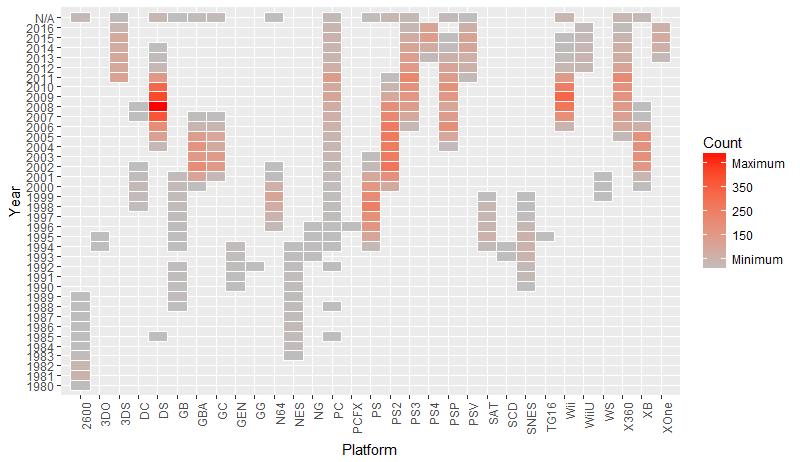
\includegraphics[scale=0.75]{Rplot07}

Na tomto grafu můžeme nejen sledovat životnost jednotlivých konzolí, ale táke úspěch jednotlivých generací. Zde je opět naprosto zjevné že předchozí generace byla ta  nejúspěšnější. Zjistili jsme také, že:

\begin{itemize}
\item Největší počet nejůspěšnějších titulů vzniká vždy uprostřed životního cyklu platformy.

\item V datasetu jde skvěle vidět, jak se generace konzolí prolínají (Atari 2600 -> Nintendo NES) a známe značky se vyvíjí (Sony Playstation -> Sony Playstation 4).

\item Životnost herní platformy (Nepočítaje osobní počítače.) je průměrně 10 let.

\end{itemize}



\newpage



\end{document}
